\documentclass{xjtureport}
\usepackage{graphicx}
\usepackage{float}
% =============================================
% Part 0 Edit the info
% =============================================

\major{大数据管理与应用}
\name{郅啸淇}
\title{最优化第二次作业}
\stuid{2184114639}
\college{管理学院}
\date{\zhtoday}
\lab{寝室}
\course{最优化理论与算法II}
\instructor{Xiangyu Chang}
\grades{??}
\expname{第二次作业题}
\exptype{完成作业}
\partner{Nobody}

\begin{document}
% =============================================
% Part 1 Header
% =============================================
\makecover

\makeheader

% =============================================
% Part 2 Main document
% =============================================

\section{HW1}
将原题中的限制条件$\sum_{j=1}^{n} x_{ij} = a_{i}, \sum_{i=1}^{m} x_{ij} = b_{j}$

转化为$I_{1*n}^{T} x_{ij} = a_{i}, I_{1*m}^{T} x_{ij} = b_{j}$

定义$\textbf{C}= \begin{bmatrix}
    C_{11} &...  & C_{1n}\\ 
     ...& ... & ...\\ 
     C_{m1}& ... &C_{mn} 
    \end{bmatrix}, 
    \textbf{x}= \begin{bmatrix}
        x_{11} &...  & x_{1n}\\ 
         ...& ... & ...\\ 
         x_{m1}& ... &x_{mn} 
        \end{bmatrix}$

则原函数$\sum_{i=1}^{m} \sum_{j=1}^{n} x_{ij}C_{ij} = \textbf{C}_{m*n}^{T}\textbf{x}_{m*n}\textbf{I}_{n*1}$

则原问题变为
\begin{equation}
    \begin{aligned} \label{P}
        & \min_{x} \textbf{C}_{m*n}^{T}\textbf{x}_{m*n}\textbf{I}_{n*1}\\
        &\begin{array}[]{r@{\quad}r@{}l@{\quad}l}
        s.t.& x_{ij} \geq 0\\
            & I_{1*n}^{T} x_{ij} = a_{i} \\
            & I_{1*m}^{T} x_{ij} = b_{j} \\
        \end{array}
    \end{aligned}
\end{equation}
\section{HW2}

\subsection{Lagrange Dual Problem and KKT Conditions}
$L(x,\lambda, v) = C^{T}x+v^{T}(Ax-b)-\lambda x$

$g(\lambda,v)= \mathop{inf}\limits_{x} L(x,\lambda,v) = -v^{T}b, if (C + A^{T}v-\lambda) = 0$

Lagrange Dual Problem
\begin{equation}
    \begin{aligned} \label{P}
        & \max_{\lambda,v} -\textbf{v}^{T}b\\
        &\begin{array}[]{r@{\quad}r@{}l@{\quad}l}
        s.t.& C+A^{T}v \geq 0\\
        \end{array}
    \end{aligned}
\end{equation}

$\bar{x} = diag(x),\bar{\lambda} = diag(\lambda)$

KKT Conditions
$\left\{
    \begin{matrix}
    &  C+A^{T}v -\lambda = 0 \\ 
    &  Ax -b = 0 \\ 
    &  x \geq 0 \\ 
    &  \lambda \geq 0 \\ 
    &   \bar{x}\bar{\lambda}\textbf{1}= 0
\end{matrix}
\right.$

\subsection{Strong Duality}
因为$\lambda \geq 0$,所以$L(x,\lambda,v)$为凸。取符合KKT条件的$(x^{*},\lambda^{*},v^{*})$,因为原问题为凸,则由定理得$(x^{*},\lambda^{*},v^{*})$为原问题和对偶问题最优点并且$d^{*} = p^{*}$,故强对偶成立。

\section{HW3}

\subsection{KKT Condditions}

$L_{\mu} (x,\lambda) = C^{T}x - \mu \sum_{i} log x_{i} +v^{T}(Ax-b)$

$\frac{\partial L_{\mu}}{\partial x} = C - \mu(\sum \frac{1}{x} + v^{T}A) = 0$


Define:$\lambda_{i} = \frac{\mu}{x_{i}}, \mu = \lambda_{i}x_{i}$

KKT Conditions$\left\{\begin{matrix}
    &  C+A^{T}v -\lambda = 0 \\ 
    &  Ax -b = 0 \\ 
    &   \bar{x}\bar{\lambda}\textbf{1}= \bar{mu} \textbf{1}
   \end{matrix}\right.$

\subsection{Secant Equation}
Define:$r_{1} = C-\lambda + v^{T}A,r_{2} = Ax -b,r_{3} =  \bar{x}\bar{\lambda}\textbf{1}- \bar{\mu}\textbf{1}$

$F(x,\lambda, v) = \begin{pmatrix}
    r_{1}\\ 
    r_{2}\\ 
    r_{3}
    \end{pmatrix}$

Secant Equation:
$F(x^{t},\lambda^{t},v^{t}) - \nabla F(x^{t},\lambda^{t},v^{t})(\begin{pmatrix}x^{t}\\ \lambda ^{t}\\ v^{t} \end{pmatrix} - \begin{pmatrix}x\\ \lambda \\ v \end{pmatrix}) = 0$

Explicit Form:
$\begin{pmatrix} C-\lambda ^{t} +v^{T}A\\ Ax^{t} - b\\ \bar{x}\bar{\lambda}\textbf{1} - \bar{\mu} \textbf{1}\end{pmatrix} - \begin{pmatrix} 0 & -1 & A\\ A &0  &0 \\  \bar{\lambda} &\bar{x}  &0 \end{pmatrix}\begin{pmatrix} \Delta x\\ \Delta \lambda \\ \Delta v \end{pmatrix} = 0$
\section{HW4}
\subsection{Standard Form}

\begin{equation}
    \begin{aligned} \label{P}
        & \min_{x_{1},x_{2},x_{3},x_{4}} -5x_{1}-x_{2}+0x_{3}+0x_{4}\\
        &\begin{array}[]{r@{\quad}r@{}l@{\quad}l}
        s.t.& x_{1} + x_{2} + x_{3} = 5\\
            &2x_{1} + \frac{1}{2} x_{2} + x_{4} = 8\\
            &x_1, x_2,x_3, x_4 \geq 0
        \end{array}
    \end{aligned}
\end{equation}
\subsection{Implement of Simplex method}
\lstinputlisting[language=Python]{code/Simplex Method2.py}

\begin{figure}[H]
\centering
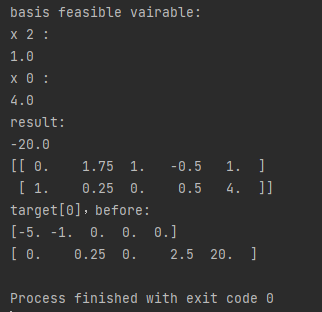
\includegraphics[scale = 0.6]{Simplex Method Result.png}
\caption{Result of Simplex Method}
\end{figure}


\subsection{Implement of Interior Point method}
\lstinputlisting[language=MATLAB]{code/Interior Point Method.py}
\begin{figure}[H]
    \centering
    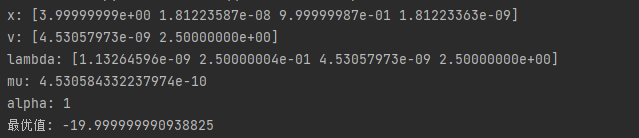
\includegraphics[scale = 0.6]{Interior Point Method.png}
    \caption{Result of Interior Method}
    \end{figure}
\section{HW5}
\lstinputlisting[language=Python]{code/HW5.py}
\begin{figure}[H]
    \centering
    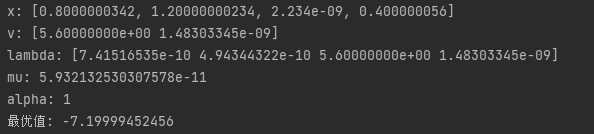
\includegraphics[scale = 0.6]{Interior Point Method2.png}
    \caption{Result of Interior Method}
    \end{figure}
\end{document}
